\chapter{Исследовательская часть}

В данном разделе приведены технические характеристики устройства, на котором проводилось измерение времени работы программного обеспечения, а также результаты замеров времени.

\section{Технические характеристики}
Характеристики используемого оборудования:
\begin{itemize}
    \item[---] операционная система --- Windows 11 Home;
    \item[---] память --- 16 Гб;
    \item[---] процессор --- 12th Gen Intel(R) Core(TM) i7-12700H @  2.30 ГГц~\cite{intel}.
\end{itemize}

\section{Цель исследования}

Целью исследования является определение зависимости времени генерации тела вращения от количества сегментов и от количества точек на кривой.

\section{Результаты замеров}

Замеры времени  проводились на одной кривой и с использованием библиотеки $QElapsedTimer$~\cite{qelapsedtimer}. Каждое значение получено путем взятия среднего из 20 измерений. Зависимость времени генерации тела вращения от количества точек на кривой представлено на рисунке~\ref{fig:point_time_mes} и замерялась с константным числом сегментов, равным 50. Зависимость времени генерации тела вращения от количества сегментов представлено на рисунке~\ref{fig:seg_time_mes} и замерялась с константным числом точек на кривой, равным 50.

\begin{figure}[H]
    \centering
    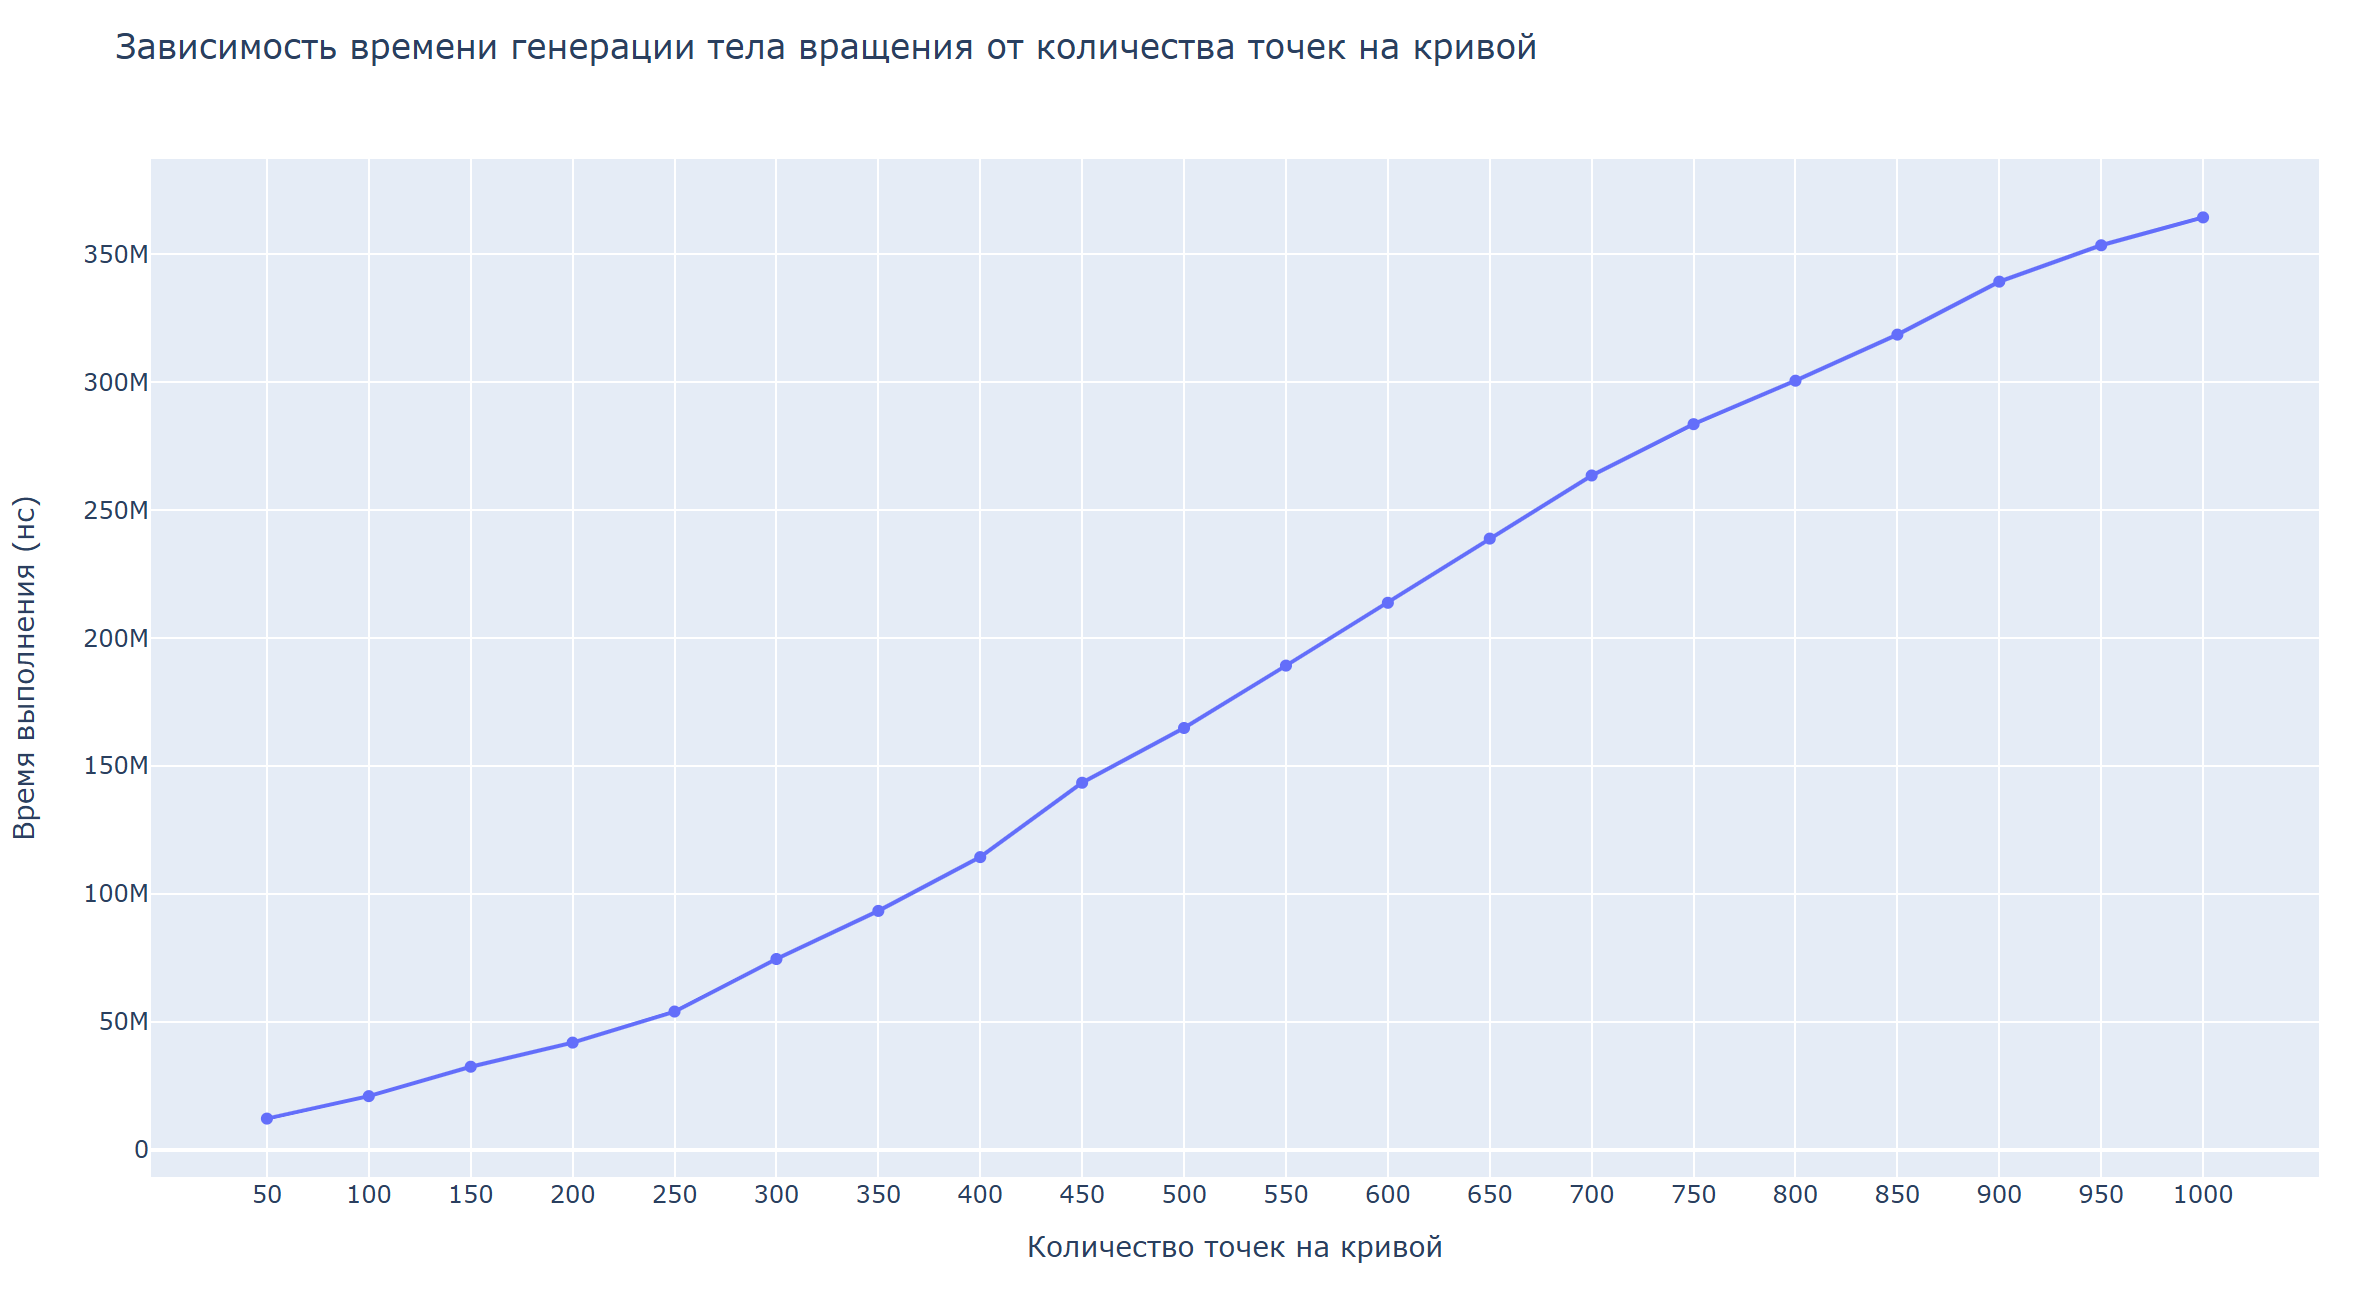
\includegraphics[width=1\linewidth]{images/plots/point_plot.png}
    \caption{Зависимость времени генерации тела вращения от количества точек на кривой}
    \label{fig:point_time_mes}
\end{figure}

\begin{figure}[H]
    \centering
    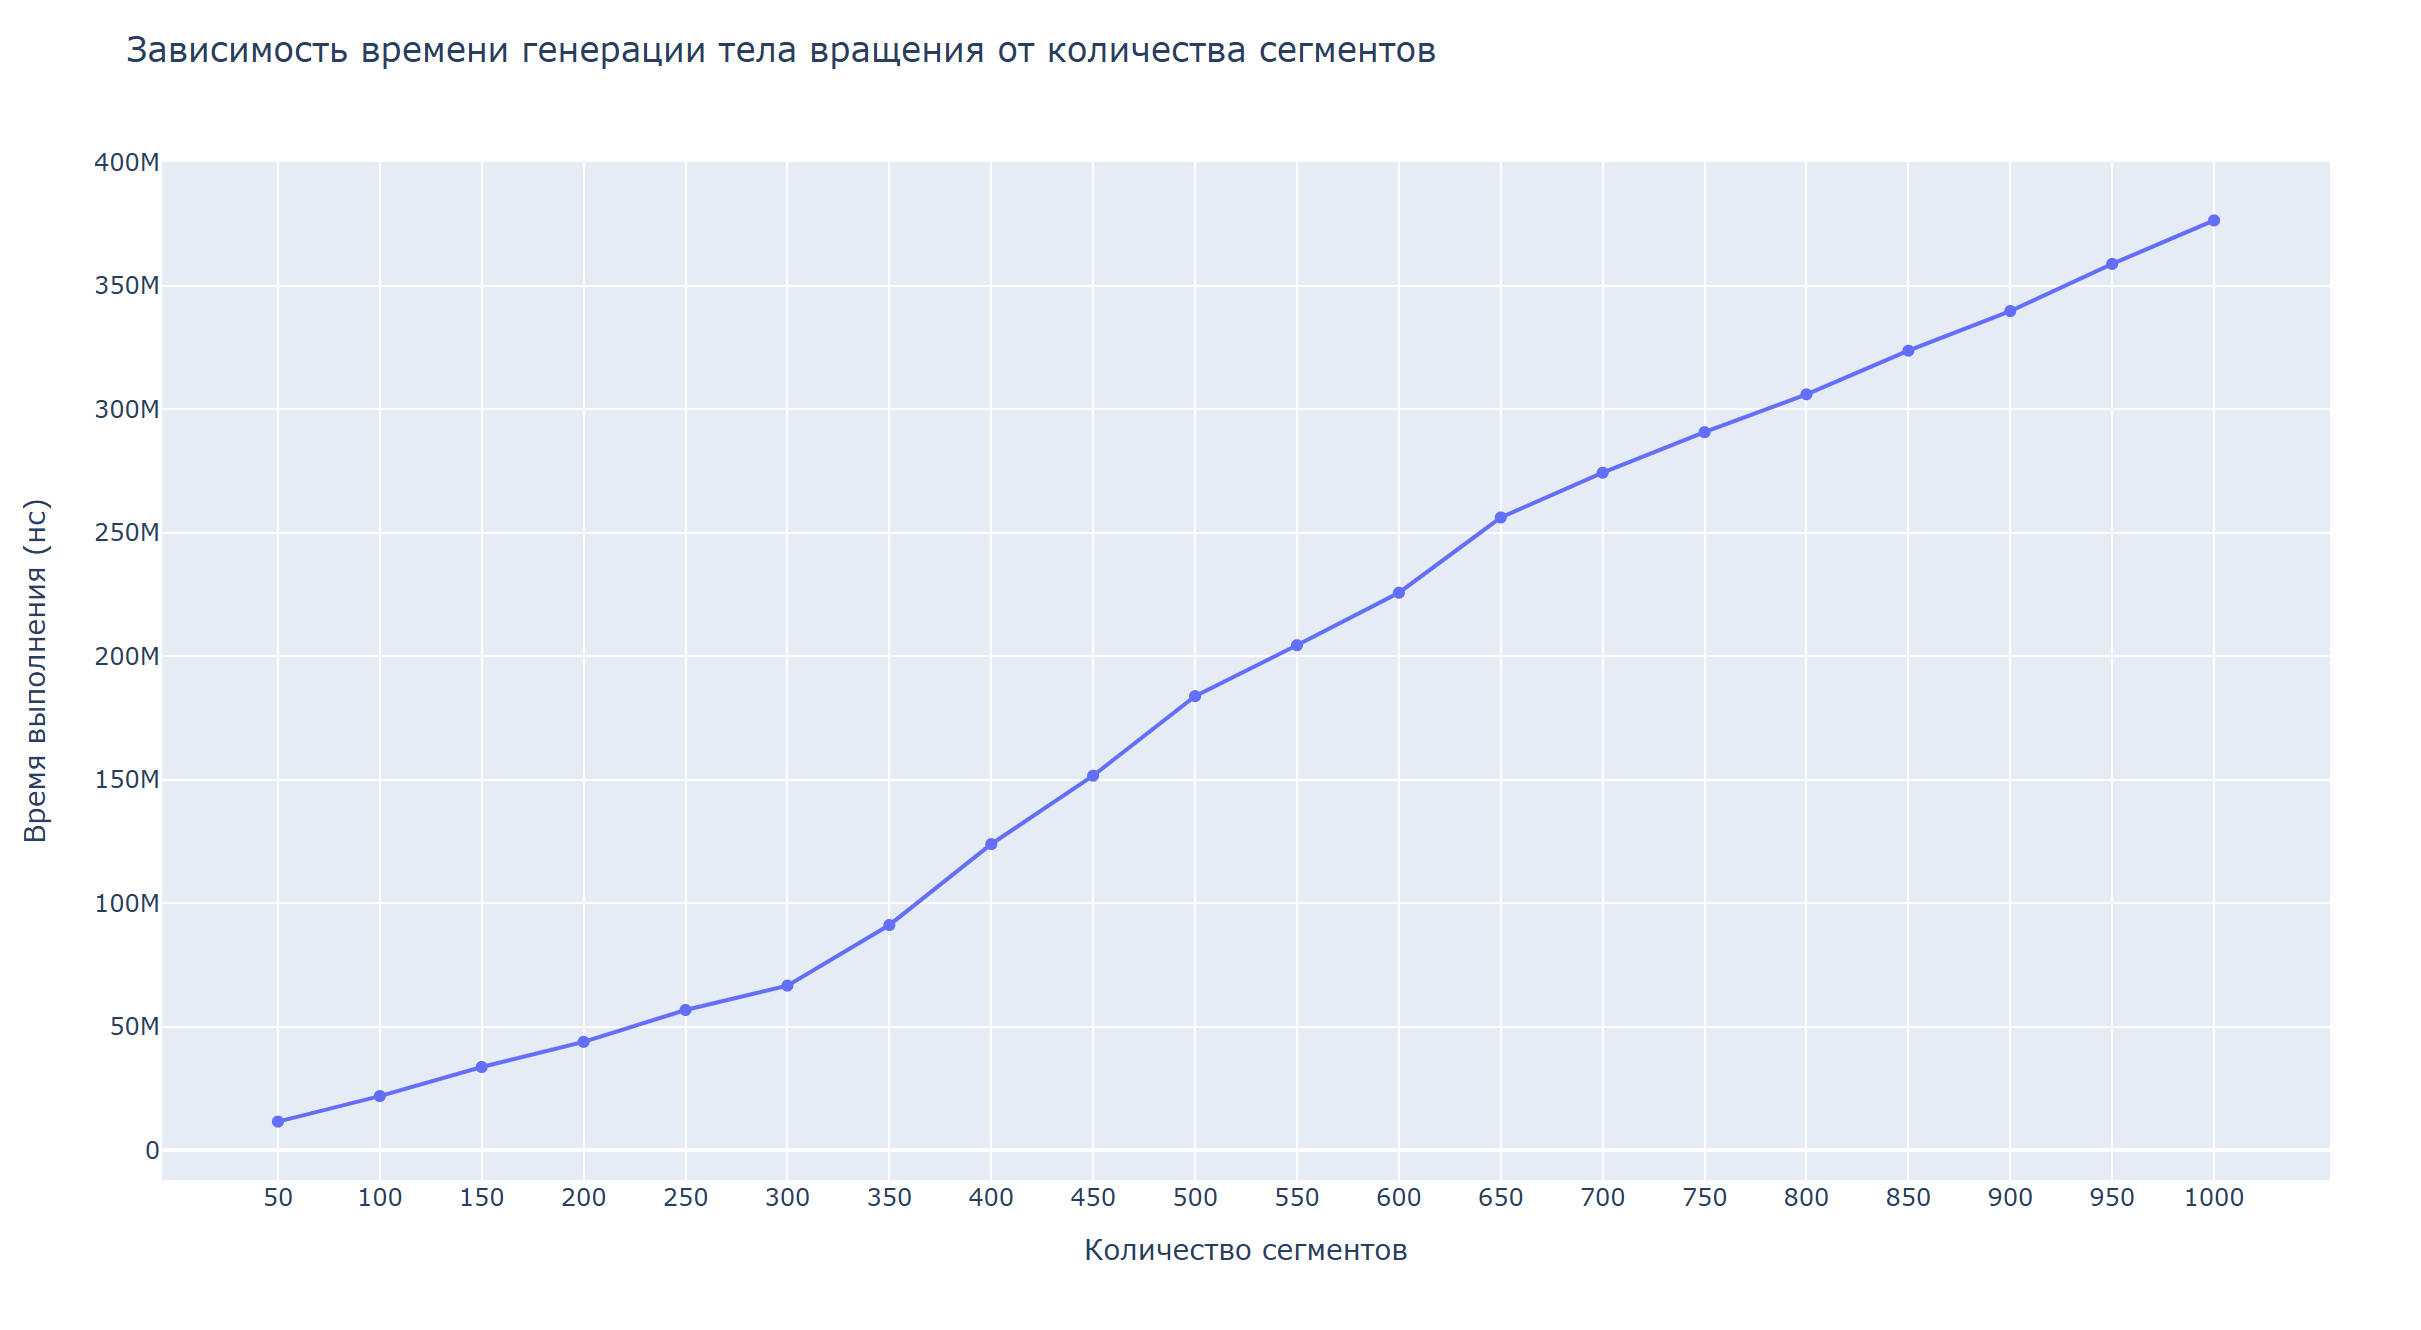
\includegraphics[width=1\linewidth]{images/plots/seg_plot.png}
    \caption{Зависимость времени генерации тела вращения от количества сегментов}
    \label{fig:seg_time_mes}
\end{figure}

\section{Результат исследования}

По результатам исследования можно сделать вывод, что зависимость времени от количества точек на кривой и от количества сегментов имеет линейный характер.

\paragraph*{ВЫВОД} ${}$ \\

В данном разделе были приведены технические характеристики устройства, на котором проводилось измерение времени работы программного обеспечения, а также результаты замеров времени.
